\documentclass[Main]{subfiles}
\begin{document}


%NUMBERING of all subsubsection ecc (in order to better grasp the quantization procedure scheme)
\setcounter{secnumdepth}{5} % seting level of numbering (default for "report" is 3). With ''-1'' you have non number also for chapters
\renewcommand\thesubsubsection{\Alph{subsubsection}}
\renewcommand\theparagraph{\thesubsubsection.\alph{paragraph}}
\renewcommand\thesubparagraph{\theparagraph.\Roman{subparagraph}}

\chapter{Geodesic Fields}
	%mettere nell'intro una breve introduzione al problema geodetico nell'approccio standard della geometria riemmaniana
	In the context of differential geometry, \emph{geodesic curves} are a generalization of \emph{straight lines}  in the sense of self-parallel curves.\\
	%Definizione di geodetica su varietà con connessione
	Considering a differential manifold $M$ endowed with an affine connection $\nabla$ we define:
	\begin{definition}[Geodesic]
		A smooth curve $\gamma:[a,b]\rightarrow M$ such that:
		\begin{equation}
			\nabla_{\dot{\gamma}}\dot{\gamma} =0
		\end{equation}
		where $\dot{\gamma}^\mu \coloneqq \frac{d \gamma^\mu}{d t}$ is the tangent vector to the curve.
	\end{definition}
	

		In local chart the previous equation assumes the well-known expression:
		\begin{equation}\label{GeodesicEquation}
			\ddot{\gamma}^i + \Gamma^i_{\, j k} \dot{\gamma}^j \dot{\gamma}^k = 0
		\end{equation}
		where $ \Gamma^i_{\, j k}$ is the coordinate representation of the Christoffel symbols of the connection.
		Equation (\ref{GeodesicEquation}) admits a well-posed Cauchy problem.
		\begin{theorem}
			Let $M$ be a smooth manifold, $p\in M$, $v \in T_p M$. 
			Then there exist $\epsilon>0$ and precisely one geodesic
			\begin{displaymath}
				c: [0,\epsilon]\rightarrow M
			\end{displaymath}
			with $c(0) = p , \dot{c}(0) = v$.\\
			 In addition, $c$ depends smoothly on $p$ and $v$.
		\end{theorem}
		\begin{proof}
		Equation \ref{GeodesicEquation} is a system of second order ODE, and the Picard-Lindelof theorem yields the local existence and uniqueness of a solution with prescribed initial values and derivatives, and this solution depends smoothly on the data.
		\end{proof}

	\vspace{4mm}
	%Definizione metrica di geodetica su varietà riemmaniana( con connessione di levi civita)	
	In presence of a pseudo-Riemannian metric it is possible to present the geodesic %in a metric sense i.e. 
	as the curve extremizing the \emph{Energy Functional}\footnote{Remember that for arc-length parametrized curves the Energy functional coincides with the length functional.\cite[Lemma $1.4.2$ ]{Jost2005}}:
	\begin{definition}[Energy functional]
  	\begin{equation}\label{EnergyFunctional}
  		H: C^1\left(\left[a,b\right],Q\right) \rightarrow \Real \qquad
 		H(\gamma) \coloneqq \int_a^b \left\Vert \frac{d \gamma}{dt} (t)\right\Vert^2 dt
 	\end{equation}
\end{definition} 	
	Considering only the proper variations (that keep the end-point fixed), the extremum condition corresponds to equation \ref{GeodesicEquation} where $\nabla$ is the unique Levi-Civita connection (torsion-free and metric-compatible).

	\vspace{4mm}
		%Problema di Jacobi, deviazione geodetica e legame alla curvatura
	In general relativity the problem of the 
	linearization of the geodesic equation yields the Jacobi equation which takes
	%geodesic equation linearization, named \emph{Jacobi equations} takes
	 a central role. \footnote{Usually in this context takes the name of \emph{Geodesic deviation} problem\cite[pag. 46]{Wald1984} inasmuch Jacobi field describes the difference between the geodesic and an "infinitesimally close" geodesic.}
	
	\begin{definition}[Jacobi Field]
	We call a \emph{Jacobi field} along the geodesic $\gamma$ the tangent vector field over the submanifold $\gamma(t,\tau)$, determined by  a smooth one parameter family of geodesics$ \gamma_\tau$ ( with $\gamma_0=\gamma$), in respect to the$\tau$ coordinate. \textit{i.e.}:
	\begin{displaymath}
	 J = \left. \frac{\partial \gamma_\tau (t)}{\partial \tau}\right\rvert_{\tau=0}
	\end{displaymath}
	\end{definition}
	
		In local charts, a Jacobi field along the geodesic $\gamma$ is solution of a linear O.D.E.:
		\begin{equation}\label{JacobiEquationComponents}
			\big( X''\big)^\mu + R^\mu_{i \alpha \j} T^i X^\alpha T^j =0
		\end{equation}
		where:
		\begin{itemize}
			\item $\big(X'\big)^\mu \coloneqq \big( \nabla_{\dot{\gamma}(t)} X\big)^\mu$ is the covariant derivative along the curve $\gamma$.
			\item $T \equiv \dot{\gamma}(t)$ stands for the tangent vector to $\gamma$.
			\item $R^\mu_{i \alpha \j}$ are the representation in components of the Riemann curvature tensor,
		\end{itemize}

	
	
	
	
	The rest of this chapter will be devoted to discussing geodesic and Jacobi fields
	% the presentation of the approach to geodesic and Jacobi problem 
	as a physical system.


\section{Geodesic Problem as a Mechanical Systems}\label{GeodesicMechanics}
	% Da quanto detto in introduzione ha un odore molto forte il legame  dell'equazione geodetica con l'equazione del moto di un punto su una varietà e dell' funzionale lunghezza come versione con il prinicpio di minima azione
	The basic idea is very simple, to portray the geodesic curve as the natural motion of a free point particle constrained on the Pseudo-Riemannian manifold $Q$.
	
	\begin{remark}
	In terms of general relativity this problem can be instantly recognized as the derivation of the motion of free-falling particles.
	
	However, there is no lack of alternative viewpoints .
	The framework of the classical \emph{geometric mechanics} taught us to picture the "static" configurations of a constrained, complex, classical system as a point on the \emph{Configuration space}.% manifold. 
	According to that, the geodesic motion can be seen as a realization of a particular dynamics on a mechanical system with a pseudo-Riemannian configuration space\footnote{Such systems can be depicted as "geodesic" even in presence of a position-dependant potential.\cite[Cap 3.7]{Abraham1978}}.
	\end{remark}


	% Q è la varietà riemmanian in esame, eccc. vedi pag 223  e successive del fomm (direi di dare per assodato tutto il contesto di meccanica geometrica che mi sono studiato nei primi mesi della tesi ma credo non sia il caso di mettere per esteso qui, al massimo solo linkarlo

	\begin{proposition}[Geodesic Motion]
		The geodesics on the Pseudo-Riemannian manifold $(Q,g)$ are the natural motions of the ordinary Lagrangian system $(Q, L)$ where:
		\begin{equation}
			L(V_q) \coloneqq \frac{1}{2} g_q(V,V)
		\end{equation}
	\end{proposition}	
	\begin{proof}
		%	 The Euler-Lagrange equation of $L$ coincides with the geodesic equation \ref{GeodesicEquation}.
		%	 \danger.. è sul quaderno non so se metterla (ho dovuto staccare i foglio per portarmeli a lecce!) ora sono pinzati al quanderno 2
		A direct computation of the Euler-Lagrange equations:
		\begin{displaymath}
			\frac{d}{dt} \left( \frac{\partial L}{\partial V^i}\right) = \frac{\partial L}{\partial q^i}
		\end{displaymath}
		for the Lagrangian
		\begin{displaymath}
			L = \frac{1}{2} g_{i j} ( \vec{q} ) V^i V^j
		\end{displaymath}
		brings to the following equation motion:
		\begin{displaymath}
			g_{k j} \ddot{q}^j = \left(
				 \frac{1}{2} \left(
				 	\frac{\partial g_{i j}}{\partial q^k} \dot{q}^i \dot{q}^j \right)
				  - \frac{\partial g_{k j}}{\partial q^i} \dot{q}^i \dot{q}^j  \right)
		\end{displaymath}
		Multiplying for the inverse of the metric we find:
		\begin{displaymath}
			g^{l k} g_{k j } \ddot{q}^j \equiv \ddot{q}^l = \frac{1}{2} g^{l k} \left( \frac{\partial g_{i j}}{\partial q^k} - \frac{\partial g_{k j}}{\partial q^i}- \frac{\partial g_{k i}}{\partial q^j}\right) \dot{q}^i \dot{q}^j 
			= - \Gamma^l_{\, i j} \dot{q}^i \dot{q}^j
		\end{displaymath}
		where in the last equation we have recognized the expression of Christoffel symbols in term of the Riemannian metric.
	\end{proof}

%	\begin{observation}
	\begin{remark}
		The geodesic system is not simply Lagrangian but also Hamiltonian.
		This property follows from the hyperregularity\cite{Abraham1978} of $L$.
	\end{remark}
%	\end{observation}

	%Qualsiasi sistema di mqo come il precedente può essere visto come un sistema campo.
	As shown in chapter 2, every system with discrete degrees of freedom can be seen as a trivial field system.
	From that it follows the alternative characterization of geodesics as a Lagrangian field:
	\begin{corollary}[Geodesic field]
		The geodesics on the Pseudo-Riemannian manifold $(Q,g)$ can be seen as the \emph{Dynamical Configurations} of the Lagrangian field system $(E,\Lagrangian)$ where:
		\begin{itemize}
			\item $E=(Q\times\Real, \pi, \Real)$ trivial smooth bundle on the real line.
			\item $\Lagrangian[\gamma] = \frac{1}{2} g(\dot{\gamma},\dot{\gamma})(t) dt$
		\end{itemize}
	\end{corollary}
	\begin{proof}
		It is a simple application of the correspondence seen in chapter \ref{MechanicsAsAField}.
	\end{proof}
	
	From this perspective it is clear that the Energy Functional corresponds to the action of the geodesic field dynamics and equation \ref{GeodesicEquation} is nothing more than the equations of motion according to the \emph{least action principle}.

% \danger aggiungere!!!
%		\begin{figure}[h!]
%		 \centering
   	%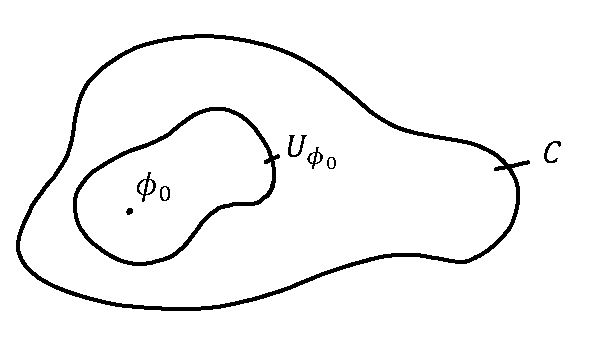
\includegraphics[width=0.5\textwidth]{Pictures/Linearization} 
   	% (credo sia la figura pagina 1 del quaderno 2)
%	 	 \caption{Impressionistic view of the geometric mechanics structure.}
%		\end{figure}		


\section{Peierls Bracket of the Geodesic field}
	The local coordinate expression for the Lagrangian density of the geodesic field is:
	\begin{equation}
		\Lagrangian\big(t,\gamma^i(t), \dot{\gamma}^i(t) \big)\coloneqq \frac{1}{2}g_{\mu,\nu}\left(\gamma^i\left(t\right)\right)\dot{\gamma}^\mu \dot{\gamma}^\nu
	\end{equation}		
	which is highly non-linear. \\
	It is explicitly is quadratic in the velocity components $\dot{\gamma}^i$ and implicitly, through $g_{\mu\nu}(\gamma^i(t))$, is non-polynomial in the %curve 
	coordinates $\gamma^i$.
	
	As show in section \ref{Section:NonLinearPeierls}, for this type of systems the calculation of the Peierls bracket can be realized only locally around a predetermined solution.
	Let us repeat the Peierls' procedure for the system under investigation.

	As a consequence of our introduction on the geodesic as a field, we can state the unperturbed dynamic as a L.P.D.O :
		\begin{equation}
			Q_\Lagrangian \big(q^\mu 	\big)= \biggr[\ddot{q}^\mu + \Gamma^\mu_{\, i j}\dot{q}^i \dot{q}^j	\biggr]
		\end{equation}
	where $\dot{q}^\mu = \frac{d}{dt}q^\mu(t)=\dot{q}^i\partial_i q^\mu$.
	
	A linear variation of $q_0^\mu +\epsilon \eta^\mu$ constructed from the coordinate representation $q_0^\mu$ of the geodesic $\gamma_0 \in \Sol$, solves the original equations of motion when
	\begin{equation}\label{GeodesicJacobation1}
		Q_\Lagrangian \big( q_0^\mu +\epsilon \eta^\mu \big) = \frac{d^2}{dt^2}\biggr( q_0^\mu +\epsilon \eta^\mu \biggr) +
		\biggr[ \Gamma^\mu_{\, i j}\big( \vec{q_0} + \epsilon \vec{\eta}\big) \biggr]\biggr(\dot{q_0}^i +\epsilon \dot{\eta}^i \biggr)\biggr(\dot{q_0}^j +\epsilon \dot{\eta}^j \biggr) = 0 \mbeq o(\epsilon)
	\end{equation}
	If we consider only the first order in the parameter $\epsilon$ we can expand the expression of the Christoffel symbols:
	\begin{displaymath}
		\biggr[ \Gamma^\mu_{\, i j}\big( \vec{q_0} + \epsilon \vec{\eta}\big) \biggr] =
		\biggr[ \Gamma^\mu_{\, i j}( \vec{q_0}) + \epsilon \eta^\alpha\big( \partial_\alpha  \Gamma^\mu_{\, i j} \big)\biggr\vert_{\vec{q_0}} + o(\epsilon) \biggr]
	\end{displaymath}	 
	
	Collecting all the terms in equation \ref{GeodesicJacobation1} up to the first order in $\epsilon$ it follows a condition on the perturbation:
	\begin{align}\label{Eq:JacobiPeierlsEquation}
	0 &= \ddot{\eta}^\mu + \eta^\alpha\big( \partial_\alpha  \Gamma^\mu_{\, i j} \big)\biggr\vert_{\vec{q_0}} \dot{q_0}^i \dot{q_0}^j  +  \Gamma^\mu_{\, i j} \big(\dot{\eta}^i \dot{q_0}^j + \dot{q_0}^i \dot{\eta}^j \big)= \nonumber \\
	&=\biggr\{ g^\mu_{\,\alpha} \frac{d^2}{dt^2} +
	 \Gamma^\mu_{\, i \alpha}(\vec{q_0})\big[2 \dot{q_0}^i \frac{d}{dt} \big] + 
\big[ \partial_\alpha \Gamma^\mu_{\, i j}(\vec{q_0}) \dot{q_0}^i \dot{q_0}^j  \big] \biggr\} \eta^\alpha	= P^\mu_{\: \alpha} \eta^\alpha
	\end{align}		
	where $ P^\mu_{\: \alpha}$ is a linear partial differential operator acting on the \emph{variations} \textit{,i.e.,} the components of a field along the geodesic $\gamma_0$.\\
	As showed in section \ref{Section:NonLinearPeierls}, equating the linearized dynamics operator with the term $-\left(Q_\chi(\gamma_0)\right)(x)$ 	(see equation \ref{PeierlJacobiEqNonLin}) leads to the inhomogeneous \emph{Jacobi operator} from which all the standard construction of the brackets Peierls follows.

	
	\begin{proposition}
		The differential equation $$P^\mu_{\: \alpha} \eta^\alpha=0$$ corresponding to the l.p.d.o $P$ defined in equation \ref{GeodesicJacobation1} corresponds to equation \ref{JacobiEquationComponents} defining  the \emph{Jacobi fields} along the geodesic $\gamma_0$.
	\end{proposition}
	\begin{proof}
		For convenience, we adopt the following notation:
		\begin{align*}
		&\eta^\mu \partial_\mu \coloneqq X \equiv X^\mu \partial_\mu \\
		&\dot{q_0}^i \partial_i \equiv \dot{\gamma_0} \coloneqq T \equiv T^i \partial_i
		\end{align*}
		We have to show that the equation just found:
		\begin{equation}\label{JacobiEqI}
			\ddot{X}^\mu + X^\alpha\left(\partial_\alpha\Gamma^{\mu}_{\, i j}\right)T^i T^j + \Gamma^\mu_{\, \alpha j}\left(2 T^i \dot{X}^\alpha \right) = 0
		\end{equation}
		where $\dot{X}^\mu = \frac{d}{dt}X^\mu= T^i \partial_i X^\mu$,
		corresponds to the equation defying the Jacobi field:
		\begin{equation}\label{JacobiEqII}
			\left(X'' \right)^\mu + R^\mu_{\, i \alpha j}T^i X^\alpha T^j = 0
		\end{equation}
		where $\left(X')\right)^\mu \coloneqq \left(D_t X \right)^\mu$ and $D_t = T^i \nabla_i$ is the covariant derivative along the curve.\\
		Since:
		\begin{align}\label{JacobiEqDerivative}
			X'' &= D_t D_t X = D_t \left( \partial_\mu \left( \dot{X}^\mu + \Gamma^\mu_{\, i \alpha} T^i X^\alpha \right)\right) \nonumber \\
			&=\left( \ddot{X}^\mu + \frac{d}{dt}\left( \Gamma^\mu_{\, i \alpha} T^j X^\alpha \right) + \Gamma^\mu_{\, j \nu}T^j \dot{X}^\nu + T^j \Gamma^\mu_{\, j \nu} \Gamma^\nu_{\, i \alpha} T^i X^\alpha \right)\partial_\mu
		\end{align}
		We can write equation \ref{JacobiEqI} in term of the covariant derivative as:
		\begin{align*}
			\left(X'' \right)^\mu &=
			- \left(
			X^\alpha\left(\partial_\alpha\Gamma^{\mu}_{\, i j}\right)T^i T^j + \Gamma^\mu_{\, \alpha i}\left(2 T^i \dot{X}^\alpha \right)
			- \frac{d}{dt}\left( \Gamma^\mu_{i \alpha} T^i X^\alpha \right) - T^j \Gamma^\mu_{\, j s} \Gamma^s_{\, i \alpha} T^i X^\alpha
			\right) =\\
			&=			
			-\left(
			X^\alpha\left(\partial_\alpha\Gamma^{\mu}_{\, i j}\right)T^i T^j - \dot{\Gamma}^\mu_{i \alpha} T^i X^\alpha
			- \Gamma^\mu_{i \alpha} \dot{T}^i X^\alpha  - T^j \Gamma^\mu_{\, j s} \Gamma^s_{\, i \alpha} T^i X^\alpha				
			\right)
		\end{align*}
		remembering that the geodesic condition is still to be met:
		\begin{displaymath}
			\dot{T}^i = - \Gamma^I_{\, j k} T^j T^k
		\end{displaymath}
		we can conclude that:
		\begin{align*}
			\left(X'' \right)^\mu &=
			- \left(
			  X^\alpha\left( \partial_\alpha\Gamma^\mu_{\, i j}\right)T^i T^j
			- T^j \left( \partial_j \Gamma^\mu_{\, i \alpha}\right) T^i X^\alpha
			+X^\alpha \Gamma^\mu_{\, \alpha s} \Gamma^s_{\, i j}T^i T^j 
			- T^j \Gamma^\mu_{\, j s} \Gamma^s_{\, i \alpha} T^i X^\alpha
			\right) =\\
			&=	-\left( R^\mu_{\, i \alpha j}T^i X^\alpha T^j\right)		
		\end{align*}
	\end{proof}
	
	

	
	

\subsection{Example: Geodesic field on FRW space-time.}
	\begin{Warning}
	% qui i conti li devo ancora fare, 
	l'idea è che le metriche possono essere diagonalizzate risulta un sistema di equazioni del moto ode disaccoppiate di cui posso calcolare la funzione di green come indicato nelle dispense che trattano il calcolo di green per le ode.
	se ho l'operatore di green posso calcolare in esplicito le soluzioni perturbate e quindi le peierls.
	Guardare pag 5 advance + pag 6 primer	
	\end{Warning}
	

\section{Algebraic quantization of the Geodesic Field}
	The algebraic quantization scheme applies only to %linear field systems.
	systems of linear fields.
	Since equation\ref{GeodesicEquation} is highly non linear,  it is not the geodesic system that can actually be quantized but rather its linearization, the Jacobi field along a fixed geodesic $\gamma_0$.
	
		\subsubsection{Classical Framework}
			The basic idea is that, chosen a geodesic $\gamma_0$, the kinematical configurations of the Jacobi fields are tangent fields along the fixed curves.
			\paragraph{Kinematics}	
			The configuration bundle $E$ corresponds to the \emph{Pull-back bundle} $\gamma_0^*(TQ)$ of the tangent bundle along the geodesic $\gamma_0$.
			Then:
			\begin{itemize}
				\item $E$ is a vector bundle over $\Real$.
				\item The base manifold $\Real$ can be considered as a degenerate globally hyperbolic spacetime, $\CauchyClass(\Real) = \Real$.
				\item the fibers are $E_p \coloneqq T_{\gamma_0(p)}Q$
				\item $\Conf = \Gamma^\infty(E) = \mathfrak{X}(\gamma_0)$ is constituted by vector fields along the curve $\gamma_0$.
			\end{itemize}
			
			\paragraph{Dynamics}
				The coordinate representation of the motion equation is:
				\begin{displaymath}
					\left( P X \right)^\mu = (X'')^\mu + R^\mu_{\, i \alpha j } T^i T^j X^\alpha
				\end{displaymath}
				where $X\in \Conf$ and $T^i = \dot{\gamma_0}^i$.
				According to equation \ref{Eq:NormallyHyperbolicRepresentation} this operator falls exactly in the class of \emph{normally hyperbolic} operators hence it is quantizable both by  means of Peierls procedure and by means of initial data.
		
		\subsection{PreQuantum Framework}
		\subsubsection{Peierls approach}
			\paragraph{Pairing}
				%The choice of the inner product on this configuration bundle is rather obvious.
				Since $Q$ is a Riemannian manifold and $\Conf$ is composed by tangent vector fields, it is straightforward to choose as inner product on the configuration bundle $E$ the metric function defined on $Q$:
				\begin{equation}
					\left\langle X,Y \right\rangle_t \coloneqq g\left( X\left(\gamma_0(t) \right),Y\left(\gamma_0(t) \right)\right)
					\qquad \forall X,Y \in E_t
				\end{equation}
				
				It follows slavishly the definition of a pairing:
				\begin{equation}
					\left( X, Y \right) = \int_\Real \left\langle X,Y \right\rangle_t dt
				\end{equation}
				well-defined for every pair $X,Y \in \Conf$ such that $\supp(X) \cap \supp(Y)$ is compact.
				
				The operator $P$ ruling the dynamics is formally self-adjoint:
				\begin{align*}
				 ( Y, PX) &= \int Y_\mu PX^\mu dt= 
				 \int\left( Y_\mu \ddot{X}^\mu + Y_\mu R^\mu_{\, i \alpha j}T^i T^j X^\alpha \right)dt = \\
 				 &= \int\left( \ddot{Y}_\mu X^\mu + X_\mu R^\mu_{\, i \alpha j}T^i T^j Y^\alpha \right)dt =
				 \int P Y_\mu X^\mu dt=( PY, X) 				 				 
				\end{align*}
				where we have integrated by parts twice (the boundary value being null since the integrand is compactly supported) and we have exploited the curvature tensor identity:
				\begin{equation}\label{Eq:CurvatureSimmetry}
					\langle R(X,T)T,Y \rangle = \langle R(Y,T)T,X \rangle
				\end{equation}

			\paragraph{Classical Observables}
				Replicating what has been done in the general case, 
				we construct the \emph{pre-observables} as the functionals $F_f:\Conf \rightarrow \Real$ for all $f \in \Gamma_0(E)$ compactly supported fields along the geodesic $\gamma_0$:
				\begin{equation}
					F_f(X) = \int_\Real <X, f>_t dt \qquad \forall X \in \Conf
				%	F_f(X) = \int_{\dom(\gamma_0)} <X, f>_t dt \qquad \forall X \in \Conf
				\end{equation}
				The space of classical observables is then obtained through the usual quotient:
				\begin{displaymath}
					\Obs \simeq \frac{\Gamma_0}{P \Gamma_0}
				\end{displaymath}
				The observables functionals are the maps:
				\begin{displaymath}
				 F_{[f]}(X) = F_f (X) \qquad \forall X \in \Sol
				\end{displaymath}
				where $f$ is a representative of the equivalence class $[f]\in \Obs$.
			
			\paragraph{Symplectic Structure}
				The geodesic motion is a particular case of a system with finite degrees of freedom, thus the Peierls brackets between two Lagrangian functionals $\chi, \omega$ around a geodesic $\gamma_0$ tested on a function $f \in C_0^\infty(\Real)$ are given by \ref{EspressionePeierlsCampiCurve}.
				Restricting the definition to the simplest Lagrangian functionals constructible from the classical observables:
				\begin{displaymath}
					\chi [\phi] \coloneqq (\chi, \phi) \qquad \chi \in \Obs,\, \phi \in \Sol
				\end{displaymath}
				corresponding to Lagrangian densities in the form:
				\begin{displaymath}
					\chi ( \vec{q}i, \dot{\vec{q}}) \coloneqq < \chi, \vec{q}> = \chi^i q_i
				\end{displaymath}
				such that $ Q_\chi \gamma_0^i = \chi^i$, the Peierls brackets expression reduces to
				\begin{displaymath}
					\left\lbrace\chi , \omega \right\rbrace (\gamma_0) [f] = \int f(t) \left\langle\chi, \left(\GreenAdv - \GreenRet \right)\omega \right\rangle dt
				\end{displaymath}
				The test-function $f$ can be neglected for regular distributions.
%				For regular distribution can be neglected the test-function $f$.

				\vspace{3.5mm}
				We conclude that,according to the Peierls' procedure,  the classical symplectic space is the pair $(\Obs, \tau)$ where:
				\begin{displaymath}
					\tau( [\chi], [\omega]) = \{\chi , \omega \} =\int \left\langle\chi, \left(\GreenAdv - \GreenRet \right)\omega \right\rangle dt = ( \chi, E \omega) \qquad \forall \chi,\omega \in \Gamma_0(E)
				\end{displaymath}
				
				
		\subsubsection{Initial data Approach}
			\paragraph{Classical Phase Space}
				The base manifold for the configuration bundle under examination is the real line $\Real$ that can be seen as a degenerate globally hyperbolic spacetime.
				Thus each point $p\in \Real$ is a Cauchy surfaces and no further support condition can be imposed.\\
				Considering that the operator $P$ is of second order, we have:
				\begin{displaymath}
					\Phase(p) \equiv \Data(p) = \Gamma^\infty(p) \times \Gamma^\infty(p) =
					T_{\gamma_0(p)}Q \times T_{\gamma_0(p)}Q
				\end{displaymath}
				and
				\begin{displaymath}
					\Phase \simeq \Sol
				\end{displaymath}
				using the map which yields the unique solution starting from an initial data.
				
			\paragraph{Symplectic Structure on the Phase Space}		
				The general definition \ref{Def:InitialDataSymplecticForm} of the symplectic form on the classical phase space reduces to:
				\begin{displaymath}
					\Omega: \Phase(p) \times \Phase(p) \rightarrow \Complex \qquad : \qquad 					
					\Omega \biggr\{ [V_0,V_1] , [W_0, W_1] \biggr\} = g(V_1,W_0)  - g( V_0, W_1) 
				\end{displaymath}
				where $g$ is the inner product on $Q$.
				\\
				This formula can be transferred to the space of solutions:
				\begin{displaymath}
					\sigma_p: \Sol \times \Sol \rightarrow \Complex \qquad : \qquad 					
					\sigma_p \biggr\{X, Y  \biggr\} = \Omega \biggr\{ [Y(t), D_t Y(t)] , [X(t), D_t X(t)] \biggr\}
				\end{displaymath}
				\vspace{3mm}
				Mimicking what has been done in example \ref{Ex:IndipendentPhaseSpace} for the scalar field, the independence of the phase space construction from the particular choice of $p \in \Real$ can be proved.\\
				Taken $X,Y \in \Sol$ two Jacobi fields on $\gamma_0(t)$, a scalar field over $\Real$ can be defined:
				\begin{displaymath}
					J(t) \coloneqq \Omega \biggr\{ [Y(t), D_t Y(t)] , [X(t), D_t X(t)] \biggr\}
					= X^\alpha(t) g_{\alpha \beta} D_t Y^\beta(t) - 
					Y^\alpha(t) g_{\alpha \beta} D_t X^\beta(t) 					
				\end{displaymath}
				where $D_t = T^\mu \nabla_\mu$ as usual.
				This is clearly a conserved current:
				\begin{eqnarray}
					D_t J =& (D_t X)^\alpha g_{\alpha \beta} (D_t Y)^\beta - (D_t Y)^\alpha g_{\alpha \beta} (D_t X)^\alpha + X^\alpha g_{\alpha \beta} D_t D_t Y^\beta - Y^\alpha g_{\alpha \beta} D_t D_t X^\beta = \nonumber \\
					=& X^\alpha g_{\alpha \beta} PY^\beta - Y^\alpha g_{\alpha \beta} PX^\beta - X_\beta R^\beta _{\, i \alpha j}T^i Y^\alpha T^j +Y_\beta R^\beta _{\, i \alpha j}T^i X^\alpha T^j  = 0
				\end{eqnarray}
				exploiting the conditions $\nabla_\mu g_{\alpha \beta}=0$, $PX=PY=0$ and equation \ref{Eq:CurvatureSimmetry}.\\
				Hence:
				\begin{displaymath}
				\int_p^{p'} D_t J = J(p) - J(p') = 0
				\end{displaymath}
			In others words:
			\begin{displaymath}
				\sigma_\Sigma (X, Y) = \sigma_{\Sigma'} (X, Y) 
				\qquad \forall X, Y \in \Sol \; \forall \Sigma, \Sigma' \in \CauchyClass(M)= \Real
			\end{displaymath}
			
				\vspace{3.5mm}
				In conclusion, according to the initial data procedure,  the classical symplectic space is the pair $(\Sol, \sigma)$ such that:
				\begin{displaymath}
					\sigma( X, Y) = X_\mu(\Sigma) \left( D_t Y (\Sigma)\right)^\nu - \left(D_t X(\Sigma)\right)_\mu Y^\nu(\Sigma) \qquad \forall X,Y \in \Sol
				\end{displaymath}
				where $\Sigma$ is an arbitrary point in $\Real$.

	\subsection{Comparisons}
		The two procedures yield two different classical symplectic spaces: $(\Obs,\tau)$ and $(\Sol, \sigma)$.
		We have proved in section \ref{Section:LinkBetweenQuantization} (Theorem \ref{Teo:IsomorphismBetweenTheTwoSymplectic}) that the two vector spaces are isomorphic through the map $\Xi$ realized with the causal propagator $E$ .
		Furthermore, in this case it can be proved that $\Xi$ preserves the symplectic form.
		\\
		Once again we mimic what has been done for the case of a scalar field (ex \ref{Ex:SimplettomorphismPhaseSpace}).
		Consider two compactly supported vector fields $f,h \in \Gamma_0(E)$ along $\gamma_0$	and call $X= Ef,\: T = Eh$ the corresponding Jacobi field.
		In fact from the definition of $\tau$ it follows:
		\begin{align}
			\tau\big( [f], [g] \big) =& (f, Eh) = \int_\Real f^\mu g_{\mu \nu} ( E h)^\nu dt =
					\int_\Sigma^\infty  f^\mu g_{\mu \nu} Y^\nu dt	 + 
					\int_{-\infty}^\Sigma  f^\mu g_{\mu \nu} Y^\nu dt
			\nonumber \\
			=& \int_\Sigma^\infty (P \GreenAdv f)^\mu g_{\mu \nu} Y^\nu dt	 + 
					\int_{-\infty}^\Sigma (P \GreenRet f)^\mu g_{\mu \nu} Y^\nu dt
		\end{align}
		where the integral has been decomposed by splitting the domain of integration into two subsets whose intersection has zero measure and we have exploited the properties of the retarded and advanced operators.\\
		Considering the explicit representation of the operator $P$, we can integrate by parts twice:
		\begin{align}
			&\int_\Sigma^\infty (P \GreenAdv f)^\mu g_{\mu \nu} Y^\nu dt = \int_\Sigma^\infty \left( D_t^{\,2} \GreenAdv f +R(\GreenAdv f,T)T \right)^\mu g_{\mu \nu} Y^\nu dt = \nonumber \\
			&= 
			 \int_\Sigma^\infty D_t \left( \left(D_t  \GreenAdv f \right)^\mu g_{\mu \nu} Y^\nu \right)dt -
			 \int_\Sigma^\infty \left( D_t  \GreenAdv f \right)^\mu g_{\mu \nu} \left( D_t Y \right)^\nu dt +
			 \int_\Sigma^\infty \left( R( \GreenAdv f,T)T \right)^\mu g_{\mu \nu} Y^\nu dt = \nonumber \\
			&= 
			 - \left. D_t( \GreenAdv f)^\mu g_{\mu \nu} Y^\nu \right\vert_\Sigma -
			 \int_\Sigma^\infty D_t \left( \left( \GreenAdv f \right)^\mu g_{\mu \nu} \left( D_t Y \right)^\nu \right)dt + \int_\Sigma^\infty \big(
			 (\GreenAdv f)^\mu g_{\mu \nu} (D_t^{\, 2}Y)^\nu + 
			 \left(R( \GreenAdv f,T)T \right)^\mu g_{\mu \nu} Y^\nu
			 \big) dt	=	 \nonumber \\
			 &=
			 -   \left. D_t( \GreenAdv f)^\mu g_{\mu \nu} Y^\nu \right\vert_\Sigma
			 +  \left. ( \GreenAdv f)^\mu g_{\mu \nu} (D_t Y)^\nu \right\vert_\Sigma
			 + \int_\Sigma^\infty \big(
			 (\GreenAdv f)^\mu g_{\mu \nu} (P Y)^\nu 
			 \big) dt =\nonumber \\
			 &= 
			 -   \left. D_t( \GreenAdv f)^\mu g_{\mu \nu} Y^\nu \right\vert_\Sigma
			 +  \left. ( \GreenAdv f)^\mu g_{\mu \nu} (D_t Y)^\nu \right\vert_\Sigma
		\end{align}
		where \emph{Stokes theorem} and property \ref{Eq:CurvatureSimmetry} have been used.
		\\
		Combining the two above equations one concludes that:
		\begin{align}
		\tau\big( [f], [g] \big) =& 
			 -   \left. D_t( \GreenAdv f)^\mu g_{\mu \nu} Y^\nu \right\vert_\Sigma
			 +  \left. ( \GreenAdv f)^\mu g_{\mu \nu} (D_t Y)^\nu \right\vert_\Sigma		+
		\nonumber \\
			&+ \left. D_t( \GreenRet f)^\mu g_{\mu \nu} Y^\nu \right\vert_\Sigma
			   -  \left. ( \GreenRet f)^\mu g_{\mu \nu} (D_t Y)^\nu \right\vert_\Sigma		
		 =  \nonumber\\
		=&\left. \left( E f \right)^\mu g_{\mu \nu} ( D_t Y)^\nu\right\vert_\Sigma	 
		-  \left.\left(D_t E f \right)^\mu g_{\mu \nu}  Y^\nu \right\vert_\Sigma	= \nonumber \\
		=& X_\mu(\Sigma) \left( D_t Y (\Sigma)\right)^\nu - \left(D_t X(\Sigma)\right)_\mu Y^\nu(\Sigma) \equiv \sigma( X, Y)
		\end{align}
		$(\Obs, \tau)$ and $(\Sol, \sigma)$ are isomorphic not only as vector spaces but also as symplectic spaces.

\section{Interpretations??????}
	\begin{Warning}
		Speriamo bene.. :S
	\end{Warning}

\end{document}
